\documentclass[UTF8]{article}
\usepackage[zihao=5]{ctex}		%字号设置
\usepackage[a4paper]{geometry}	%页面设置
\geometry{left=2cm,right=2cm,top=2cm,bottom=5cm}
\usepackage{graphicx} 			%插入并编辑图片
\usepackage{siunitx}			%更好看的物理单位(手打其实更快些)
\usepackage{mhchem}				%写化学公式
\usepackage{chemfig}
\usepackage{fancyhdr}			%设置页眉页脚
\usepackage{lmodern}			%一种编码字体
\usepackage{amsmath}			%数学公式扩展
\usepackage{threeparttable}		%三线表宏包1
\usepackage{booktabs}			%三线表宏包2
\usepackage{float} 
\usepackage{subfigure}
\usepackage{autobreak}
\usepackage{amsmath}
\usepackage{indentfirst}
\usepackage{tabularx}
\graphicspath{{figures/}}		%将报告中需要的图片储存于此
\pagestyle{fancy}				%设置页眉页脚
\setlength{\headheight}{70pt}
\setlength{\parindent}{2em}

\begin{document}
	\pagestyle{empty}
	\vspace*{8em}
	\begin{center}
		{\Huge 南非心脏病数据分析与建模}\\
		\bigskip  % 垂直间距
	\end{center}
	\vspace{8em}  % 垂直间距
	% 信息
	\begin{center}
		{\Large  % 这里的字号也可以用别的方式修改
			
			\makebox[3em][s]{作者}:\underline{\makebox[10em][c]{PB22010322 杨锡灿}}\\
		}
	\end{center}
	\vspace{20em}  % 垂直间距
	\begin{center}
		
		\the\year.\the\month.\the\day
	\end{center}
	\clearpage  
	\newpage
	\setcounter{page}{0}
	\begin{center}
		\tableofcontents
	\end{center}
	
	
	\newpage
	\pagestyle{fancy}	
	\fancyhead[L]{中国科学技术大学《机器学习方法》课程}
	\rhead{南非心脏病数据分析与建模}
	\section{关键词}
	偏差分析、统计特征生成、热力图、随机森林、支持向量机(SVM)、XGBoost、K 近邻算法、超参数优化、交叉验证、决策边界
	\section{摘要}
	心脏病是全球范围内的主要公共健康问题之一,早期预测和干预对降低发病率具有重要意义。本研究以南非心脏病数据为基础,利用数据分析与机器学习技术构建心脏病预测模型。通过数据清洗、特征工程和可视化,揭示了各变量之间的关系,并利用偏差分析筛选出对心脏病预测具有显著影响的特征。接着,分别使用随机森林、支持向量机(SVM)、XGBoost 和 K 近邻算法进行建模,再进行超参数优化之后,通过交叉验证评估模型性能。最终根据准确率、F1 分数和 ROC AUC三个指标的综合表现选择 SVM 作为最佳模型。在最后的结果呈现中,该模型能够有效识别高风险群体,为心脏病的早期筛查提供了一种高效、可靠的工具。本研究为基于机器学习的心脏病预测提供了有益探索,并具备实际应用价值。
	\section{引言}
	\subsection{背景介绍}
	心血管疾病(Cardiovascular Disease, CVD)是全球范围内导致死亡的主要原因之一,尤其在发展中国家,其发病率和致死率逐年上升。在南非,心血管疾病的负担尤为显著,受到不健康的生活方式、遗传因素以及不平等医疗资源分布的多重影响。尽管如此,对于心血管疾病风险因素的全面分析和精准建模仍存在许多研究空白。\\
	\indent 为了降低心血管疾病的发病率,早期风险评估至关重要。传统的风险预测多基于单一或少数变量,例如高血压、胆固醇水平等。然而,这种方法往往忽略了多个风险因素的交互作用。在现代数据驱动时代,机器学习等先进的建模方法为分析复杂疾病提供了强有力的工具,可以结合多维数据,捕捉潜在的风险模式。\\
	\subsection{研究目标}
	研究的目标是构建一个具有良好预测性能的心血管疾病风险评估模型,以期为疾病预防和公共卫生干预提供科学依据。\\
	
	\newpage
	\section{数据描述、预处理及可视化}
	\subsection{变量描述}
	本研究使用的数据集包括南非人群的若干生理指标、行为特征以及心血管疾病相关标签,共有以下变量:
\begin{table}[ht]
	\centering
	\caption{变量描述}
	\begin{tabularx}{\textwidth}{|l|X|l|X|}
		\hline
		\textbf{变量名称} & \textbf{变量描述} & \textbf{单位/类别} & \textbf{备注} \\ \hline
		\textbf{sbp}      & 收缩压(Systolic Blood Pressure)       & mmHg         & 心血管健康的重要生理指标,高水平与高血压相关。 \\ \hline
		\textbf{tobacco}  & 吸烟量(Tobacco Use)                  & 千克/年      & 累积吸烟量,用于衡量吸烟习惯的严重性。          \\ \hline
		\textbf{ldl}      & 低密度脂蛋白胆固醇(Low-Density Lipoprotein Cholesterol) & mmol/L      & 常被称为“坏胆固醇”,与动脉硬化密切相关。       \\ \hline
		\textbf{adiposity}& 肥胖度(Adiposity)                    & 无单位       & 一种衡量个体脂肪水平的指标,高值可能提示肥胖。  \\ \hline
		\textbf{famhist}  & 家族史(Family History of Heart Disease) & 类别("Present" 或 "Absent") & 用于反映遗传风险,心血管疾病有显著的家族聚集性。 \\ \hline
		\textbf{typea}    & A型性格分数(Type A Behavior Score)    & 分数         & 高分数通常与压力相关,可能是心脏病的心理社会风险因素。 \\ \hline
		\textbf{obesity}  & 肥胖指数(Obesity)                    & 无单位       & 根据体重和身高计算得出,用于衡量身体质量。      \\ \hline
		\textbf{alcohol}  & 酒精消费量(Alcohol Consumption)       & g/周         & 长期过量饮酒可能是心血管疾病的风险因素。        \\ \hline
		\textbf{age}      & 年龄(Age)                            & 年           & 心血管疾病的主要非可控风险因素,风险随年龄增长而增加。 \\ \hline
		\textbf{chd}      & 是否患有心脏病(Coronary Heart Disease) & 类别(0 = 无, 1 = 有) & 目标变量,用于指示是否存在心血管疾病。         \\ \hline
	\end{tabularx}
	\label{table:variables}
\end{table}
	\newpage
	\subsection{数据预处理}
	\subsubsection{数据清洗}
    经过简单的检查,本次的数据中并没有出现异常值和缺失值,所以可以跳过数据清洗工作。\\
    \subsubsection{数据降维}
受到本课程参考书 The Elements of Statistical Learning中4.4节南非心脏病例子的启发,我认为通过偏差分析剔除不显著的变量是一个良好的降维方法,所以我先保留所有的特征进行了逻辑斯蒂模型的拟合,计算全模型的偏差,之后通过逐个剔除变量,计算每个模型的偏差,最后制成了一个直观显示偏差值,偏差差异以及p值(通过偏差差异计算)的表格如下\\
    \begin{table}[ht]
    	\centering
    	\caption{变量的偏差分析}
    	\begin{tabular}{|c|c|c|c|}
    		\hline
    		\textbf{Variable} & \textbf{Deviance} & \textbf{Deviance Difference} & \textbf{p-value} \\ \hline
    		famhist   & -107.223321 & 16.745067 & 0.000043 \\ \hline
    		age       & -109.580016 & 14.388371 & 0.000149 \\ \hline
    		typea     & -113.061832 & 10.906556 & 0.000958 \\ \hline
    		tobacco   & -114.434009 & 9.534379  & 0.002017 \\ \hline
    		ldl       & -115.038297 & 8.930090  & 0.002805 \\ \hline
    		obesity   & -121.875175 & 2.093213  & 0.147955 \\ \hline
    		sbp       & -122.671273 & 1.297114  & 0.254741 \\ \hline
    		adiposity & -123.563376 & 0.405011  & 0.524512 \\ \hline
    		alcohol   & -123.967651 & 0.000736  & 0.978352 \\ \hline
    	\end{tabular}
    	\label{table:deviance_analysis}
    \end{table}

\noindent 注:考虑到famhist数据类型的不便处理,我将数据集中famhist数据的absent和present替换为了0和1\\

去除掉p值大于0.05的变量,我们再进行同样的操作以确定是否还有需要进一步剔除的变量,得到表格如下
\begin{table}[ht]
	\centering
	\caption{变量的偏差分析(2)}
	\begin{tabular}{|c|c|c|c|}
		\hline
		\textbf{Variable} & \textbf{Deviance} & \textbf{Deviance Difference} & \textbf{p-value} \\ \hline
		age       & -93.729590   & 26.693252 & 2.384528e-07 \\ \hline
		famhist   & -104.013581  & 16.409261 & 5.103526e-05 \\ \hline
		tobacco   & -110.076216  & 10.346626 & 1.297115e-03 \\ \hline
		typea     & -110.664559  & 9.758283  & 1.785166e-03 \\ \hline
		ldl       & -111.394085  & 9.028757  & 2.657651e-03 \\ \hline
	\end{tabular}
	\label{table:deviance_analysis}
\end{table}
	\subsection{特征工程}
	为了方便后续建模,我将要用的的几个变量数据进行了特征化,得到了'age\_scaled', 'ldl\_scaled', 'tobacco\_scaled','typea\_scaled'这几个变量,之后我们通过这几个变量进行分析和建模。   
	\subsection{数据可视化}
	\subsubsection{相关性热力图}
	图a展示了选定特征之间的相关性热力图。通过计算 Pearson 相关系数,我们可以直观地看到变量之间的关系。例如,age\_scaled 和 tobacco\_scaled 之间呈现较强的正相关,这有助于识别特征间的关联性。
	\begin{figure}[htbp]
		\centering
		% 第一张图片
		\subfigure[相关性热力图]{
			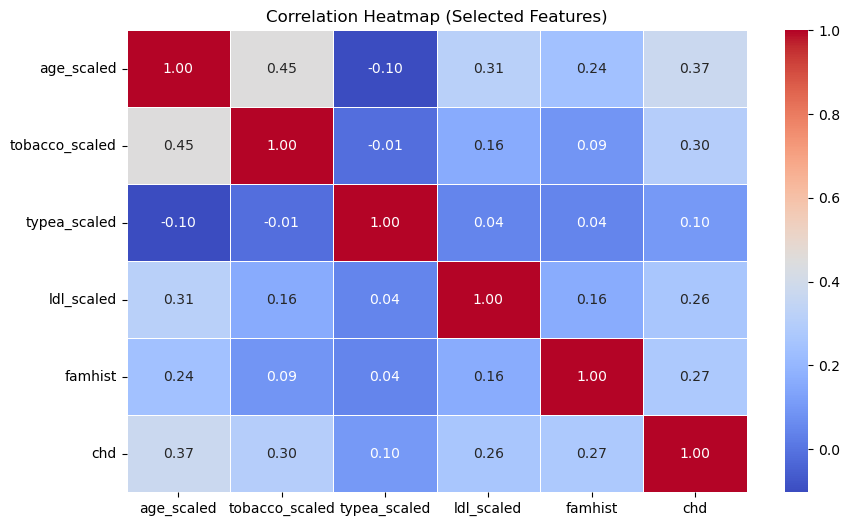
\includegraphics[width=0.45\textwidth]{1.png}
		}
		% 第二张图片
		\subfigure[散点图矩阵]{
			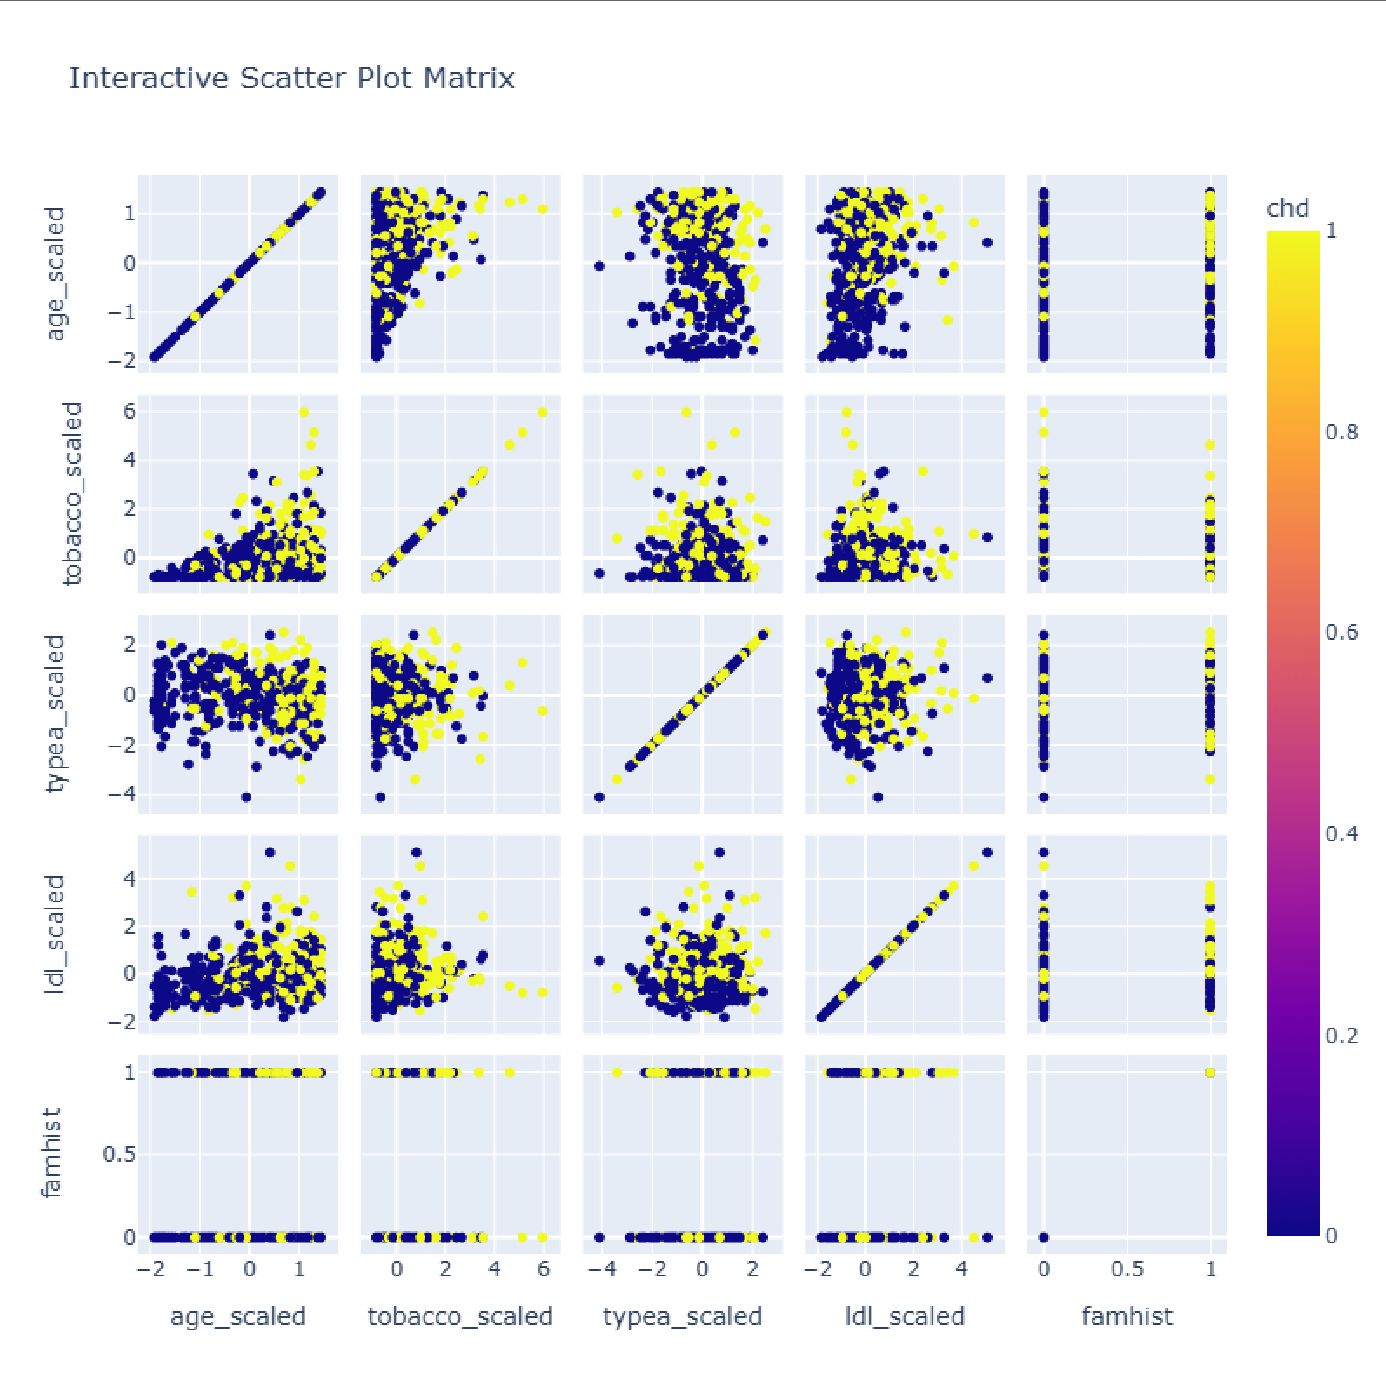
\includegraphics[width=0.3\textwidth]{2.png} 
		}
	\end{figure}
	\subsubsection{散点图矩阵}
 图b是一个交互式散点图矩阵,展示了选定特征与心脏病(chd)之间的关系。通过颜色标识,用户可以查看不同变量组合下的分布情况,便于识别潜在的模式和群体结构。
	\section{建模方法}
	\subsection{备选模型介绍}
	首先明确到这是一个分类问题,我们需要通过数据集建立模型,再利用模型通过'age\_scaled', 'ldl\_scaled', 'tobacco\_scaled','typea\_scaled'这些变量预测心脏病,所以我初步的地选择了以下几个建模方法
	\subsubsection{随机森林}
	随机森林是一种集成学习方法,基于多个决策树的组合。它通过在训练集上随机选择样本和特征来构建多个决策树,并通过投票或平均的方法得到最终的预测结果。每棵树都是独立的,因此可以有效避免单一决策树的过拟合问题。\\
	选择理由:南非心脏病数据中的特征可能对心脏病的影响存在复杂的非线性关系,随机森林能够有效捕捉这些复杂的特征交互。
	\subsubsection{支持向量机}
	 支持向量机是一种通过找到最大间隔超平面(最大化类间边界)来进行分类的算法。SVM 使用核技巧(例如线性核、径向基核等)来将数据映射到高维空间,在这个空间中线性可分。它主要通过支持向量来进行训练,仅利用最重要的数据点(支持向量)来决定分类边界。\\
	 选择理由:本次的数据只有462条,并不多,SVM可能达到更好的效果。
	\subsubsection{XGBoost}
	XGBoost 是一种基于梯度提升树(Gradient Boosting Tree, GBT)的集成方法。它通过迭代训练决策树,并通过减少每一轮迭代的残差来优化模型。XGBoost 具有高效的计算性能,支持正则化,有助于避免过拟合。\\
	选择理由:计算性能高效。
	\subsubsection{K近邻算法}
	K近邻算法(KNN)是一种基于实例的学习方法,通过计算待分类数据点与训练数据集中每个点的距离,然后选择距离最近的 K 个点,通过这些点的多数类别来决定预测类别。KNN 是懒惰学习算法,不需要训练过程,直接根据数据计算。\\
	选择理由:KNN 对数据的局部区域非常敏感,如果心脏病的发生与特定特征的局部模式有较强关联,KNN 会有较好的表现。
	\subsection{模型选择}
	\subsubsection{超参数选优}
	为了发挥出每个建模方法的最大功效,我决定先利用GridSearchCV对这四个模型进行超参数调优,得到以下四组超参数:\\
	Random Forest Best Params: \{'max\_depth': 3, 'min\_samples\_leaf': 2, 'min\_samples\_split': 2, 'n\_estimators': 100\}\\
	SVM Best Params: \{'C': 0.1, 'gamma': 'scale', 'kernel': 'linear'\}\\
	XGBoost Best Params: \{'learning\_rate': 0.01, 'max\_depth': 3, 'n\_estimators': 200, 'subsample': 0.8\}\\
	KNN Best Params: \{'metric': 'manhattan', 'n\_neighbors': 7, 'weights': 'uniform'\}
	\subsubsection{评估指标}
	在比较模型之前,我需要先介绍一下我评估模型使用的几个指标:\\
	\noindent 准确率 (Accuracy):预测正确的样本占总样本的比例。\\
	选择理由:准确率是最常见的分类评估指标,适用于数据集中的类别分布比较均衡的情况。在心脏病预测中,准确率能够直观地反映出模型整体的分类效果。如果心脏病的正负类别分布较均衡,那么准确率是一个有效的度量标准。\\
	
\noindent F1 分数 (F1 Score):精确率(预测为正的准确性)和召回率(正样本被识别的比例)的调和平均值。\\
	选择理由:在医学领域的分类问题中,尤其是心脏病预测,正负类样本常常存在不平衡。F1 分数综合考虑了模型的精确度和召回率,因此对于不均衡数据集更为有用。在心脏病预测中,我们通常希望能够尽量少地错过心脏病患者(提高召回率),同时也希望预测的结果是准确的(提高精确度)。F1 分数能够平衡这两个目标,特别是在正负类分布不均的情况下。\\
	
	\noindent ROC AUC:ROC 曲线下的面积,衡量模型在不同阈值下的整体性能,值越接近 1 越好。\\
	选择理由:ROC AUC 能够在不同的决策阈值下评估模型的性能,因此不依赖于特定的分类阈值(如 0.5)。它可以有效评估模型在正负类样本不平衡的情况下的表现。对于心脏病预测任务,我们可能并不总是选择 0.5 作为阈值,尤其是在处理不平衡数据时。通过 ROC AUC,我们可以更全面地理解模型的分类能力。
	\subsubsection{模型评估和筛选}
	在选定好要使用的超参数后,通过交叉验证对这四个模型进行评估,得到结果如下。
	\begin{table}[ht]
		\centering
		\caption{模型评估指标对比}
		\begin{tabular}{|l|c|c|c|}
			\hline
			\textbf{模型}        & \textbf{Accuracy (Mean ± Std)} & \textbf{F1 (Mean ± Std)} & \textbf{ROC AUC (Mean ± Std)} \\ \hline
			Random Forest & $0.7295 \pm 0.0460$          & $0.5137 \pm 0.0774$      & $0.7719 \pm 0.0354$           \\ \hline
			SVM           & $0.7295 \pm 0.0184$          & $0.5544 \pm 0.0309$      & $0.7801 \pm 0.0130$           \\ \hline
			XGBoost       & $0.7424 \pm 0.0413$          & $0.5538 \pm 0.0865$      & $0.7710 \pm 0.0291$           \\ \hline
			KNN           & $0.7035 \pm 0.0426$          & $0.5067 \pm 0.0741$      & $0.7371 \pm 0.0295$           \\ \hline
		\end{tabular}
		\label{tab:model_comparison}
	\end{table}

	根据表中数据,支持向量机(SVM)在ROC AUC 均值上取得了最高值($0.7801$),这表明其在正负样本的区分能力上最为出色。同时,SVM 在 F1 分数($0.5544$)中也表现良好,且标准差最低($0.0309$),展现了较高的稳定性。尽管 XGBoost 在 Accuracy 均值 上略高于 SVM($0.7424$ 对比 $0.7295$),但其在其他指标上的优势并不明显,且稳定性略逊。K近邻(KNN)模型的所有指标均低于其他三种模型,因此可以直接排除。而随机森林(Random Forest)尽管在 ROC AUC 上有一定的表现,但其 F1 分数 和 Accuracy 均低于 SVM 和 XGBoost,且标准差较大,表现出较低的稳定性。\\
	\indent 综合考虑模型性能指标和稳定性,我认为支持向量机(SVM)是本次南非心脏病数据建模的最佳模型,因为SVM 不仅在 ROC AUC 指标上表现最佳,还在 F1 分数 和稳定性方面展现了良好的平衡性。作为备选方案,XGBoost 也表现出色,尤其是在准确率方面稍优于 SVM。如果未来需要优化对准确率的关注,或数据集进一步扩展至更复杂的特征集,XGBoost 将是一个值得考虑的模型选择。
	\newpage
	\section{建模结果可视化}
	在确定选择SVM建模之后,我通过4:1划分数据集为训练集和测试集以训练模型,以下是对训练结果的可视化:
	\subsection{决策边界图 (Decision Boundary)}
	这张图展示了通过主成分分析(PCA)将数据降维到二维后,SVM 模型的决策边界。决策边界分隔了不同类别的预测区域,表示模型如何将输入特征映射到不同类别。在图中,训练集和测试集的样本点被分别标记为圆圈和叉号,颜色对应于类别标签。该图帮助我们直观地理解 SVM 模型如何区分不同的类别。
	\begin{figure}[h]
		\centering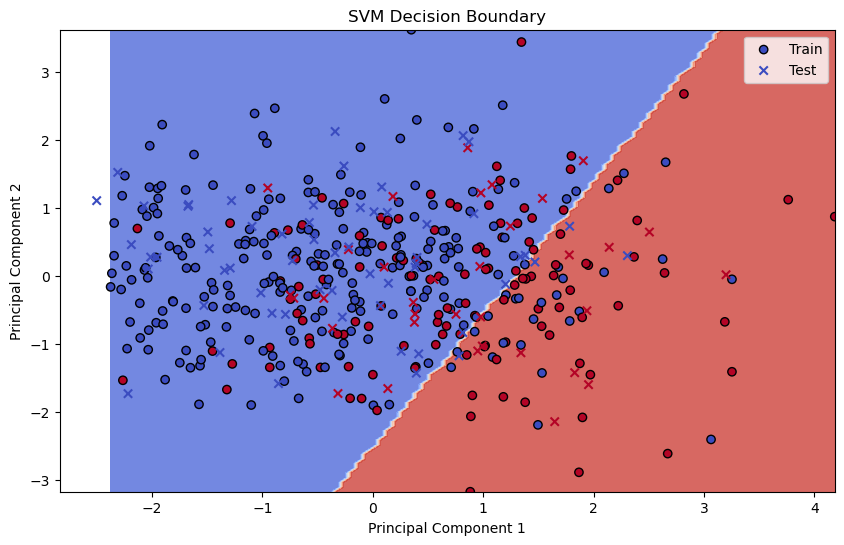
\includegraphics[width=0.5\linewidth]{3.png}
	\end{figure}
	\subsection{ROC 曲线图 (ROC Curve)}
	这张图展示了模型在不同阈值下的性能。ROC 曲线(接收者操作特征曲线)描绘了假阳性率(FPR)与真正率(TPR)之间的关系。曲线下面积(AUC)是评估模型分类能力的常用指标,AUC 值越大,表示模型的性能越好。曲线越接近左上角,模型的表现越好。
	\begin{figure}[h]
		\centering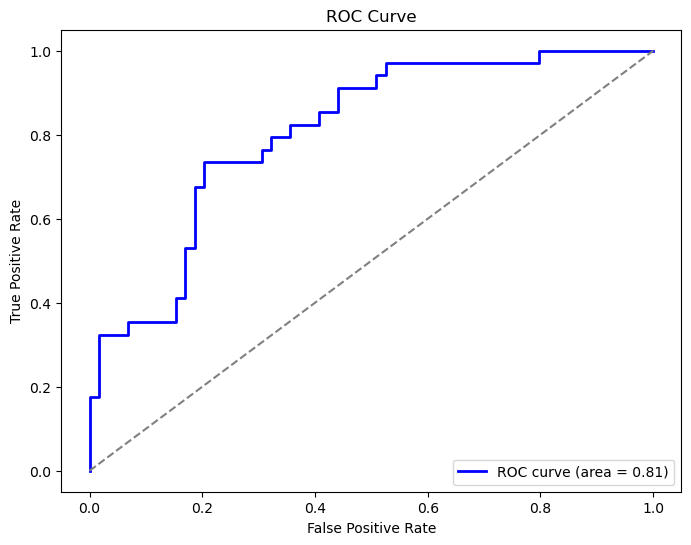
\includegraphics[width=0.5\linewidth]{4.png}
	\end{figure}
	\subsection{混淆矩阵 (Confusion Matrix)}
	混淆矩阵用于评估分类模型的性能,通过显示预测类别与实际类别的对比。在这张图中,每个格子表示模型在测试集上的分类结果。对于二分类问题,矩阵的四个元素通常是:真正(True Positive)、假正(False Positive)、真负(True Negative)和假负(False Negative)。通过分析混淆矩阵,能够识别模型在不同类别上的准确性和误分类情况。
	\begin{figure}[h]
		\centering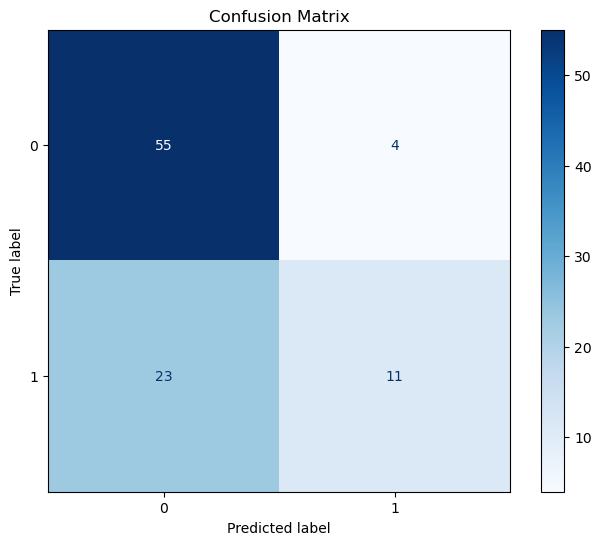
\includegraphics[width=0.5\linewidth]{5.png}
	\end{figure}
	\section{结论}
	本研究通过分析南非心脏病数据并使用支持向量机(SVM)模型进行建模,成功地构建了一个心脏病预测模型。结果表明,SVM模型在准确率和ROC AUC指标上表现优异,能够有效识别高风险群体。该模型的实际应用前景广阔,可以用于早期筛查、个性化健康管理以及公共卫生规划。通过早期识别潜在的心脏病患者,医疗机构可以采取及时干预措施,从而降低疾病发生率,减轻医疗负担。此外,该模型的成功应用不仅限于心脏病预测,还可以扩展到其他慢性病的早期诊断,为健康管理提供更加精准的决策支持。
\end{document}